% Copyright (c) 2010 Andrew Brown <brownan@cs.duke.edu, brownan@gmail.com>
% This is the source to a presentation I gave on decoding Reed-Solomon
% codes.
% Compile with: latex presentation.tex && dvips -O 0.0,0.1 presentation.dvi && ps2pdf presentation.ps
% (or see compile.sh)
% Download a compiled copy from:
% http://www.cs.duke.edu/courses/spring10/cps296.3/decoding_rs.pdf
\documentclass[]{prosper}
\usepackage[leqno]{amsmath}
\usepackage{graphicx}
\title{Implementing Reed-Solomon}
\author{Andrew Brown}

\begin{document}
\maketitle

\begin{slide}{Recall}
\begin{itemize}
\item Reed-Solmon represents messages as polynomials and over-samples them for redundancy.
\item An $(n, k, n-k+1)$ code has
    \begin{itemize}
    \item $k$ digit messages
    \item $n$ digit codewords
    \item $n-k+1$ distance between codewords (at least)
    \item $(n-k)/2$ errors before it cannot be decoded
    \item $2s = n-k$
    \end{itemize}

\item In this presentation, all messages and codewords are over the finite field $GF(2^8)$. This makes byte-oriented implementation easy
\end{itemize}
\end{slide}

\begin{slide}{Recall}
\begin{itemize}
    \item Generator Polynomial:
    \begin{itemize}
        \item $g(x) = (x-\alpha)(x-\alpha^2) \cdots (x-\alpha ^{n-k})$
        \item $\alpha$ is a generator element in $GF(2^8)$
    \end{itemize}

    \item Encoding Process:
    \begin{itemize}
        \item $m$ is the message encoded as a polynomial
        \item $m^\prime = m x^{2s}$
        \item $b = m^\prime \pmod{g}$
        \begin{itemize}
            \item $m^\prime = q g + b$ for some $q$
        \end{itemize}
        \item $c = m^\prime - b$
    \end{itemize}
    \item Codewords are multiples of $g$, {\it and} are systematic
    \item Verifying a codeword is valid is a matter of checking for divisibility by $g$

\end{itemize}
\end{slide}

\begin{slide}{Decoding Procedure Overview}
\begin{enumerate}
    \item {\bf Calculate Syndromes}
    \item {\bf Berlekamp-Massey Algorithm} - calculates the Error Locator Polynomials and Error Evaluator Polynomials
    \item {\bf Chien Search} - Finds the error locations using the Error Locator Polynomial
    \item {\bf Forney's Formula} - Finds the error magnitudes using the error evaluator polynomial
    \item {\bf Correct the Errors}
\end{enumerate}
\end{slide}

\begin{slide}{Decoding (Defining Terms)}
\begin{itemize}
    \item Error Polynomial
    \begin{eqnarray*}
    R(x) &=& C(x) + E(x) \\
    E(x) &=& E_0 + E_1x + \cdots + E_{n-1}x^{n-1}
    \end{eqnarray*}
    \begin{itemize}
        \item Has at most $s$ coefficients that are non-zero
    \end{itemize}

    \item Error Positions
    \begin{itemize}
        \item $j_1, j_2, \cdots j_s$, each a value between $0$ and $n-1$
    \end{itemize}

    \item Error Locations
    \[ X_i = \alpha^{j_i} \]

    \item Error Magnitudes
    \[ Y_i = E_{j_i} \]
    \item Notice that there are $2s$ unknowns
\end{itemize}
\end{slide}

\begin{slide}{Decoding (Syndromes)}
\begin{itemize}
    \item Step 1: Calculate the first $2s$ syndromes
    \item Syndromes are defined for all $l$:
    \[ s_l = \sum_{i=1}^s Y_i X_i^l \]
    \item For the first $2s$, it reduces to:
    \[ s_l = E(\alpha ^l) = \sum_{i=1}^s Y_i \alpha^{lj_i} \quad 1 \le l \le 2s \]
    \item $s_l = R(\alpha^l) = E(\alpha^l)$ for the first $2s$ powers of $\alpha$.
    \item Equivalent to having $2s$ equations with $2s$ unknowns
\end{itemize}
\end{slide}

\begin{slide}{Decoding (Syndromes)}
\begin{itemize}
    \item Encode the syndromes in a generator polynomial:
    \[ s(z) = \sum_{i=1}^\infty s_i z^i \]
    \item This can be computed by finding each $s_i$ from the received codeword for the first $2s$ values. That's all we need though.
\end{itemize}
\end{slide}

\begin{slide}{Berlekamp-Massey Algorithm}
\begin{itemize}
    \item Input: Syndrome polynomial from the last slide
    \item Output: Error Locator Polynomial $\sigma(z)$ and Error Evaluator Polynomial $\omega(z)$. Defined as:
    \begin{eqnarray*}
    \sigma(z) &=& \prod_{i=1}^s (1 - X_i z) \\
    \omega(z) &=& \sigma(z) + \sum_{i=1}^s z X_i Y_i \prod_{\substack{j=1\\j \ne i}}^s (1 - X_j z)
    \end{eqnarray*}
    \item Notice that the error locations are the inverse roots of $\sigma(z)$. (Roots are $1/X_1, 1/X_2, \cdots 1/X_s$)
\end{itemize}
\end{slide}

\begin{slide}{B-M (The Key Equation)}
\begin{itemize}
    \item Observe the following relation:
    \begin{eqnarray*}
    \frac{\omega(z)}{\sigma(z)} &=& 1 + \sum_{i=1}^s \frac{z X_i Y_i}{1 - X_i z} \\
    &=& ... \text{intermediate steps omitted} \\
    &=& 1 + s(z)
    \end{eqnarray*}
    
    \item Key equation thus states:
    \[ (1 + s(z)) \sigma(z) \stackrel{\pmod{z^{2s+1}}}{=} \omega(z)  \]
    \item $\sigma(z)$ and $\omega(z)$ have degree at most $s$
    \item Key Equation represents a set of $2s$ equations and $2s$ unknowns
    % Omitted for space
    %\item B-M iteratively generates a series of $2s$ pairs of polynomials where the last pair is the real $\sigma(z)$ and $\omega(z)$
\end{itemize}
\end{slide}

\begin{slide}{B-M (procedure)}
\begin{itemize}
    \item B-M iterates $2s$ times
    \item At each iteration, it produces a pair of polynomials:
    \[ (\sigma_{(l)}(z), \omega_{(l)}(z)) \]
    \item where the polynomials satisfy that iteration's key equation:
    \[ (1 + s(z)) \sigma_{(l)}(z) \stackrel{\pmod{z^{l+1}}}{=} \omega_{(l)}(z)  \]
\end{itemize}
\end{slide}

\begin{slide}{B-M (procedure)}
\begin{itemize}
    \item Once we have
    \[ (\sigma_{(l)}(z), \omega_{(l)}(z)) \]
    for some $l$. If we're lucky, they already satisfy the next key equation:
    \[ (1 + s(z)) \sigma_{(l)}(z) \stackrel{\pmod{z^{(l+2)}}}{=} \omega_{(l)}(z)  \]
    in which case we can set $\sigma_{(l+1)}(z) = \sigma_{(l)}(z)$ and similarly for $\omega(z)$
    \item However, usually we have an unwanted higher-order term:
    \[ (1 + s(z)) \sigma_{(l)}(z) \stackrel{\pmod {z^{l+2}}}{=} \omega_{(l)}(z) + \Delta_{(l)} z^{l+1}  \]
\end{itemize}
\end{slide}

% This slide summarizes the rest of the algorithm so the next 5 slides
% could be skipped
\begin{slide}{B-M (procedure)}
\begin{itemize}
    \item $\Delta_{(l)}$ is the non-zero coefficient of $z^{l+1}$ in $(1 +s(z))\sigma_{(l)}(z)$
    \item Basic idea is to iteratively improve estimates of $\sigma$ and $\omega$
    \item But since there may be a higher order term, we can't always just extend to $l + 1$ from iteration $l$
    \item A complex set of rules determines how to handle different cases
    \item The next 5 slides describe these cases and how to handle them

\end{itemize}
\end{slide}

% Following slides can be omitted for brevity
\begin{slide}{B-M (Details)}
\begin{itemize}
    \item $\Delta_{(l)}$ is the non-zero coefficient in $(1 + s(z))\sigma_{(l)}(z)$
    \item To find the next iteration's polynomials, we introduce two more polynomials $\tau_{(l)}(z)$ and $\gamma_{(l)}(z)$
    \item They must satisfy:
    \[ (1 + s(z)) \tau_{(l)}(z) \stackrel{\pmod{z^{l+1}}}{=} \gamma_{(l)}(z) + z^l  \]
    \item And we have the following rules to derive the next $\sigma$ and $\omega$:
    \begin{eqnarray*}
    \sigma_{(l+1)}(z) &=& \sigma_{(l)}(z) - \Delta_{(l)}z\tau_{(l)}(z) \\
    \omega_{(l+1)}(z) &=& \omega_{(l)}(z) - \Delta_{(l)}z\gamma_{(l)}(z)
    \end{eqnarray*}
\end{itemize}
\end{slide}

\begin{slide}{B-M (Details)}
\begin{itemize}
    \item But how to compute $\tau_{(l+1)}(z)$ and $\gamma_{(l+)}(z)$?
    \item Use one of the following rules:
        \begin{align}
        \label{ruleA}
        \tau_{(l+1)}(z) &=& z\tau_{(l)}(z) \tag{A} \\
        \gamma_{(l+1)}(z) &=& z\gamma_{(l)}(z) \nonumber \\
        \label{ruleB}
        \tau_{(l+1)}(z) &=& \frac{\sigma_{(l)}(z)}{\Delta_{(l)}} \tag{B} \\
        \gamma_{(l+1)}(z) &=& \frac{\omega_{(l)}(z)}{\Delta_{(l)}} \nonumber
        \end{align}
\end{itemize}
\end{slide}

\begin{slide}{B-M (Details)}
\begin{itemize}
    \item One of (\ref{ruleA}) or (\ref{ruleB}) is chosen each iteration to minimize the degrees of $\tau_{(l+1)}(z)$ and $\gamma_{(l+1)}(z)$
    \item To choose, define a single value $D_{(l)}$ for each iteration
    \item Choose rule (\ref{ruleA}) if $\Delta_{(l)} = 0$ or $D_{(l)} > \frac{l+1}{2}$
    \item Choose rule (\ref{ruleB}) if $\Delta_{(l)} \ne 0$ and $D_{(l)} < \frac{l+1}{2}$
    \item With rule (\ref{ruleA}) set $D_{(l+1)} = D_{(l)}$
    \item With rule (\ref{ruleB}) set $D_{(l+1)} = l + 1 - D_{(l)}$
    \item These rules and conditions ensure $0 < D_{(l+1)} \le l+1$ and the degrees of $\sigma_{(l+1)}$ and $\omega_{(l+1)}$ are upper-bounded by $D_{(l+1)}$ and degrees of $\tau_{(l+1)}$ and $\gamma_{(l+1)}$ are upper-bounded by $l - D_{(l)}$
\end{itemize}
\end{slide}

\begin{slide}{B-M (Details)}
\begin{itemize}
    \item But what about when $\Delta_{(l)} \ne 0$ and $D_{(l)} = \frac{l+1}{2}$?
    \item Either rule works, but to do even better, define one last value, a binary value $B_{(l)}$, for each iteration
    \item When $B_{(l)} = 0$ use rule (\ref{ruleA})
    \item When $B_{(l)} = 1$ use rule (\ref{ruleB})
    \item With rule (\ref{ruleA}) set $B_{(l+1)} = B_{(l)}$
    \item With rule (\ref{ruleB}) set $B_{(l+1)} = 1 - B_{(l)}$
    \item This keeps the degree inequalities satisfied:
    \begin{eqnarray*}
        \operatorname{degree} \omega_{(l)}(z) &\le& D_{(l)} - B_{(l)} \\
        \operatorname{degree} \gamma_{(l)}(z) &\le& l - D_{(l)} - (1 - B_{(l)})
    \end{eqnarray*}
\end{itemize}
\end{slide}

\begin{slide}{B-M (Details)}
\begin{itemize}
    \item All those rules ensure the degrees of $\sigma$ and $\omega$ do not grow too large. Each step they satisfy:
    \begin{eqnarray*}
        \operatorname{degree} \sigma_{(l)} &\le& (l+1)/2 \\
        \operatorname{degree} \omega_{(l)} &\le& l/2
    \end{eqnarray*}
    \item Last piece: the initial conditions:
    \begin{eqnarray*}
        \sigma_{(0)}(z) &=& 1 \\
        \omega_{(0)}(z) &=& 1 \\
        \tau_{(0)}(z)   &=& 1 \\
        \gamma_{(0)}(z) &=& 0 \\
        D_{(0)}         &=& 0 \\
        B_{(0)}         &=& 0 \\
    \end{eqnarray*}
\end{itemize}
\end{slide}

\begin{slide}{Decoding: Next Steps}
\begin{itemize}
    \item Now we have the Error Locator Polynomial $\sigma(z)$ and the Error Evaluator Polynomial $\omega(z)$
    \item Chien's Search takes $\sigma(z)$ and outputs the error locations/positions ($X_i$ and $j_i$)
    \item Forney's Formula takes $\omega(z)$ and the array $X_i$ of error locations outputs the error magnitudes ($Y_i$)
\end{itemize}
\end{slide}

\begin{slide}{Chien's Procedure}
\begin{itemize}
    \item Recall the definition of $\sigma(z)$:
    \[
    \sigma(z) = \prod_{i=1}^s (1 - X_i z)
    \]
    \item Now that we have $\sigma(z)$, finding the array of $X_i$ values is simply a matter of solving for the roots
    \item The Easy Way: since we're working over a small field, just test every value
    \begin{enumerate}
        \item Let $\alpha$ be a generator
        \item Initialize $\{X_i\}$ to the empty set
        \item For $l = 1, 2, \ldots$ \\
            If $\sigma(\alpha^l) = 0$: add $\alpha^{-l}$ to $\{X_i\}$
    \end{enumerate}
\end{itemize}
\end{slide}

\begin{slide}{Chien's Procedure}
\begin{itemize}
    \item But we can do better than evaluating it 255 times!
    \item If we have computed the $\alpha^l$th evaluation, we get:
    \[ \sigma(\alpha^l) = 1 + \sigma_1\alpha^l + \sigma_2\alpha^{2l} + \sigma_3\alpha^{3l} + \cdots + \sigma_s\alpha^{sl} \]
    \item Then, computing $\sigma(\alpha^{l+1})$ is an $O(s)$ operation:
    \[ \sigma(\alpha^{l+1}) = 1 + \sigma_1\alpha^{l+1} + \sigma_2\alpha^{2l+2} + \sigma_3\alpha^{3l+3} + \cdots + \sigma_s\alpha^{sl+s} \]
    \item The $i$th term in $\sigma(\alpha^{l+1})$ can be computed from the $i$th term in $\sigma(\alpha^l)$ by multiplying that term by $\alpha^i$
\end{itemize}
\end{slide}

\begin{slide}{Forney's Formula}
    Using the Error Evaluator Polynomial $\omega(z)$ and the error locations $\{X_i\}$, the error magnitudes $\{Y_i\}$ can be computed
    \begin{align*}
    \omega(z) &= \sigma(z) + \sum_{i=1}^s z X_i Y_i \prod_{\substack{j=1\\j \ne i}}^s (1 - X_j z) \\
    \intertext{Evaluate at $X_l^{-1}$}
    \omega(X_l^{-1}) &= \sigma(X_l^{-1}) + \sum_{i=1}^s X_l^{-1} X_i Y_i \prod_{\substack{j=1\\j \ne i}}^s (1 - X_j X_l^{-1})
    %&= Y_l \prod_{\substack{j=1\\j \ne l}}^s (1 - X_j X_l^{-1} )
    \end{align*}
\end{slide}

\begin{slide}{Forney's Formula}
    \begin{align*}
    \omega(X_l^{-1}) &= \sigma(X_l^{-1}) + \sum_{i=1}^s X_l^{-1} X_i Y_i \prod_{\substack{j=1\\j \ne i}}^s (1 - X_j X_l^{-1}) \\
    \intertext{Then simplifies to:}
    &= Y_l \prod_{\substack{j=1\\j \ne l}}^s (1 - X_j X_l^{-1} )
    \end{align*}
    since $\sigma(X_l^{-1}) = 0$
\end{slide}



\begin{slide}{Forney's Formula}
    \[
    \omega(X_l^{-1}) = Y_l \prod_{\substack{j=1\\j \ne l}}^s (1 - X_j X_l^{-1} )
    \]
    Can then be solved for $Y_l$:
    \[
    Y_l = \frac{\omega(X_l^{-1})}{ \displaystyle\prod_{\substack{j=1\\j \ne l}}^s (1 - X_j X_l^{-1}) }
    \]
    And that can be directly computed. We know all the values on the right hand side!
\end{slide}

\begin{slide}{Putting it all together}
\begin{itemize}
    \item We know:
    \begin{itemize}
        \item $\{X_i\}$ The error locations
        \item $\{Y_i\}$ The error magnitudes
    \end{itemize}
    \item Put them together to build the Error Polynomial $E(x)$
    \item Then subtract to get the codeword!
    \[
        C(x) = R(x) - E(x)
    \]
\end{itemize}
\end{slide}


\begin{slide}{Reed-Solomon Implementation}
The rest of the presentation is about my implementation
\begin{itemize}
    \item Done in Python with no external libraries or dependencies
    \item Implemented a Finite Field class for $GF(2^8)$
    \item Implemented a Polynomial Class for manipulating polynomials
    \item Implemented the RS algorithms as described
\end{itemize}
\end{slide}

\begin{slide}{Finite Fields}
\begin{itemize}
    \item Created a Python class that subclasses int
    \item Instances are integers, which represent the corresponding finite field element when translated to a polynomial
    \[ 51 = 00110011 = x^5 + x^4 + x + 1 \]
    \item Overwrote addition, subtraction, multiplication, division, and exponentiation for finite field arithmetic
    \item Multiplication defined using an exponentiation table and a logarithm table, pre-generated
\end{itemize}
\end{slide}

\begin{slide}{Finite Fields (multiplication)}
\begin{verbatim}exptable = (1, 3, 5, 15, 17, 51, ... 246, 1)\end{verbatim}
\begin{itemize}
    \item This table holds all powers of 3
    \item \begin{verbatim}exptable[1] = 3\end{verbatim}
    \item \begin{verbatim}exptable[255] = 1\end{verbatim}
\end{itemize}
\begin{verbatim}logtable = (None, 0, 25, 1, 50, 2, ... 112, 7)\end{verbatim}
\begin{itemize}
    \item This table holds all logarithms in base 3
    \item \begin{verbatim}logtable[3] = 1\end{verbatim}
    \item \begin{verbatim}logtable[17] = 4\end{verbatim} (since $3^4 = 17$)
    \item \begin{verbatim}logtable[0]\end{verbatim} is an error
\end{itemize}
\end{slide}

\begin{slide}{Finite Fields (multiplication)}
\begin{verbatim}exptable = (1, 3, 5, 15, 17, 51, ... 246, 1)\end{verbatim}
\begin{verbatim}logtable = (None, 0, 25, 1, 50, 2, ... 112, 7)\end{verbatim}
\begin{itemize}
    \item These tables together define multiplication like this:
\end{itemize}
\begin{verbatim}
def multiply(a, b):
    x = logtable[a]
    y = logtable[b]
    z = (x + y) % 255
    return exptable[z]
\end{verbatim}
\end{slide}

\begin{slide}{Finite Fields (more)}
\begin{verbatim}exptable = (1, 3, 5, 15, 17, 51, ... 246, 1)\end{verbatim}
\begin{verbatim}logtable = (None, 0, 25, 1, 50, 2, ... 112, 7)\end{verbatim}
\begin{itemize}\item Exponentiation and multiplicative inverses also use these tables:\end{itemize}
\begin{verbatim}
def power(a, b):
    x = logtable[a]
    z = (x * b) % 255
    return exptable[z]

def inverse(a):
    e = logtable[a]
    return exptable[255 - e]
\end{verbatim}
\end{slide}

\begin{slide}{Polynomial Class}
\begin{itemize}
    \item Stores numbers from high degree to low degree
    \item All coefficient math is done using regular Python operators
    \item Compatible with both integers and field elements as coefficients
    \item Supports long division and remainders (essential for RS coding)
\end{itemize}
\end{slide}

\begin{slide}{Reed Solomon Encoding}
    Since the polynomial class abstracts polynomial math away, encoding boils down to basically:
\begin{verbatim}
def encode(m):
    mprime = m * xshift
    b = mprime % g
    c = mprime - b
    return c
\end{verbatim}
\end{slide}

\begin{slide}{Reed Solomon Decoding}
Decoding is also fairly simple:
\begin{verbatim}
def decode(r):
    sz = syndromes(r)
    sigma, omega = berlekamp_massey(sz)
    X, j = chien_search(sigma)
    Y = forney(omega, X)

    # There is a loop to build E here
    ...

    return r - E
\end{verbatim}
\end{slide}

\begin{slide}{Reed Solomon Decoding}
\begin{itemize}
    \item My implementation of those functions are straight up implementations of the math. Nothing surprising.
\begin{verbatim}
def syndromes(r):
    s = [GF256int(0)]
    for l in range(1, n-k+1):
        s.append(r.evaluate(GF256int(3)**l))
\end{verbatim}
    \item My Chien Search isn't actually Chien's search though, it just evaluates the polynomial 255 times:
\begin{verbatim}
    p = GF256int(3)
    for l in range(1,256):
        if sigma.evaluate( p**l ) == 0:
            X.append( p**(-l) )
            j.append(255 - l)
\end{verbatim}
\end{itemize}
\end{slide}


\begin{slide}{Implementation Notes}
\begin{itemize}
    \item Message to Polynomial translations
    \begin{enumerate}
        \item ``hello''
        \item 104, 101, 108, 108, 111
        \item $104x^4 + 101x^3 + 108x^2 + 108x^1 + 111$
    \end{enumerate}
    \item Messages are effectively left-padded with null bytes
\end{itemize}
\end{slide}

\begin{slide}{Example}
\begin{itemize}
    \item RS(20,13) code: 13 message bytes and 7 parity bytes. Can correct 3 errors.
    \item Message: ``Hello, world!''
    \item Codeword: ``Hello, world![8d][13][f4][f9][43][10][e5]''
    \item R: ``[00][00][00]lo, world![8d][13][f4][f9][43][10][e5]''
    \item Decoded: ``Hello, world!''
\end{itemize}
And, to prove this isn't faked...
\end{slide}

\begin{slide}{Demo!}
As an example, I have written a program that encodes codewords as rows in an image
\begin{itemize}
    \item Uses RS(255,223)
    \item Encodes each symbol as a pixel in a grayscale image
    \item Each row is a codeword
    \item
    
\includegraphics{encodedimage}
    \item Decodes to:
\begin{verbatim}
ALICE'S ADVENTURES IN WONDERLAND
Alice was beginning to get very tired of
sitting by her sister on the ...
\end{verbatim}
\end{itemize}
\end{slide}

\begin{slide}{Demo!}
\begin{itemize}
    \item Since each row is a RS(255,223) codeword, it can handle up to 16 pixel errors per row.
    \item Drawing 5 px stripes, each of the following still decodes:
    \item 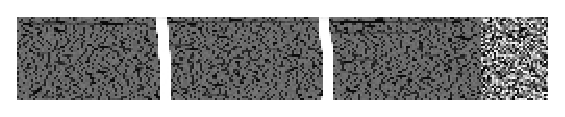
\includegraphics{encodedimage_stripes1}
    \item 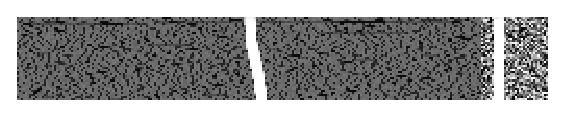
\includegraphics{encodedimage_stripes2}
    \item 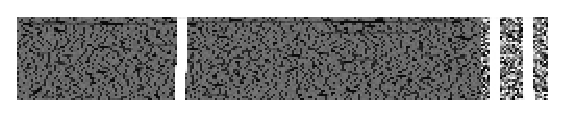
\includegraphics{encodedimage_stripes3}
\end{itemize}
\end{slide}



\end{document}
